The following sections are dedicated to the Wireless Communications Layer of this project. This layer includes the Ethernet Subsystem and the Black Box Subsystem. The Wireless Communications Layer manages the communications demands between the Web Interface Layer and the Camera Layer via UDP transport protocol over a wireless network provided the consumer by TrafficNet LLC.

\subsection{Wireless Communications Layer}
User issued commands will be sent from the Web Interface Layer to the Black Box Subsystem via UDP/IP Transfer Protocol, and subsequently forwarded by the Ethernet Subsystem to the Raspberry Pi Zero for execution.   

\subsection{Wireless Communications Layer Hardware}
Specifically, the Wireless Communications Layer is comprised of a TBD Wireless Network Adapter of TrafficNet, LLC's choosing and the Ethernet Adapter connected to the Raspberry Pi Zero. The two components work in tandem to provide a means through which the Raspberry Pi Zero can establish communication with the Web Interface Layer.

\subsection{Layer Software Dependencies}
It is necessary for the appropriate software to be present on the Raspberry Pi Zero to provide the end connection for the video streaming server to operate through. This software runs the UDP/IP Transfer Protocol which allows the video to be streamed wirelessly to the Web Interface Layer. It is the TrafficNet.py program described in the Camera Layer.

\subsection{Subsystem 1}
Descibe at a high level the purpose and basic design of this subsystem. Is it a piece of hardware, a class, a web service, or something else? Note that each of the subsystem items below are meant to be specific to that subystem and not a repeat of anything discussed above for the overall layer.

\begin{figure}[h!]
	\centering
 	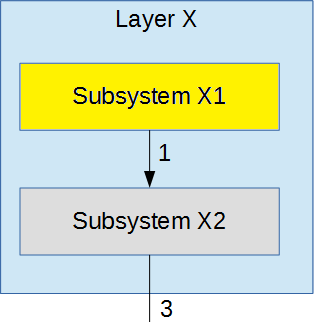
\includegraphics[width=0.60\textwidth]{images/subsystem}
 \caption{Example subsystem description diagram}
\end{figure}

\subsubsection{Subsystem Hardware}
A description of any involved hardware components for the subsystem.

\subsubsection{Subsystem Operating System}
A description of any operating systems required by the subsystem.

\subsubsection{Subsystem Software Dependencies}
A description of any software dependencies (libraries, frameworks, design software for mechanical parts or circuits, etc) required by the subsystem.

\subsubsection{Subsystem Programming Languages}
A description of any programming languages used by the subsystem.

\subsubsection{Subsystem Data Structures}
A description of any classes or other data structures that are worth discussing for the subsystem. For example, data being transmitted from a microcontroller to a PC via USB should be first be assembled into packets. What is the structure of the packets?

\subsubsection{Subsystem Data Processing}
A description of any algorithms or processing strategies that are worth discussing for the subsystem. If you are implementing a well-known algorithm, list it. If it is something unique to this project, discuss it in greater detail.


